%% ma: L12-B04-0008
%% lop: 12
%% chuong: 1
%% bai: 4
%% dang: 12.4.8
%% loai: TN4
%% muc: TH
%% dap_an: "A"
%% nguon: "(NBV)-ĐỀ SỐ 11-MỖI NGÀY 1 ĐỀ THI 2025.pdf (D11, MỖI NGÀY 1 ĐỀ - Đề số 11), Phần I Câu 1"
%% kien_thuc: "Bài 4 (đọc bảng biến thiên của hàm phân thức bậc nhất trên bậc nhất), Bài 3 (tiệm cận đứng, tiệm cận ngang), Bài 1 (đạo hàm và tính đơn điệu)"
%% trang_thai: chinh-thuc
%% ghi_chu: "Đã duyệt 13/10/2026. Đáp án gốc A đúng. Bảng biến thiên dựng lại bằng tkz-tab từ hình gốc."
\begin{ex}
Trong các hàm số dưới đây, hàm số nào có bảng biến thiên như sau?
\begin{center}
\begin{tikzpicture}
  \tkzTabInit[lgt=1.2,espcl=3.2]{$x$/.8,$y'$/.8,$y$/2.4}{$-\infty$,$-1$,$+\infty$}
  \tkzTabLine{,+,d,+,}
  \tkzTabVar{-/$2$,+D-/$+\infty$/$-\infty$,+/$2$}
\end{tikzpicture}
\end{center}
\choice{\True $y=\dfrac{2x-1}{x+1}$}{$y=\dfrac{2x+1}{x-1}$}{$y=\dfrac{x-2}{x+1}$}{$y=\dfrac{x+2}{x-1}$}
\loigiai{Bảng biến thiên cho thấy đồ thị có tiệm cận đứng $x=-1$ và tiệm cận ngang $y=2$, hàm số đồng biến trên $(-\infty;-1)$ và $(-1;+\infty)$.

Loại B và D vì có tiệm cận đứng $x=1$. Loại C vì có tiệm cận ngang $y=1$.

Với $y=\dfrac{2x-1}{x+1}$: $y'=\dfrac{3}{(x+1)^2}>0$ với mọi $x\ne-1$, $\lim\limits_{x\to\pm\infty}y=2$, phù hợp. Chọn A.}
\end{ex}
